%%%%%%%%%%%%%%%%%%%%%%%%%%%%%%%%%%%%%%%%%%%%%%%%%%%%%
%  ENTRA Deliverable
%%%%%%%%%%%%%%%%%%%%%%%%%%%%%%%%%%%%%%%%%%%%%%%%%%%%%
\documentclass[oneside]{book}


\usepackage{times} 
\usepackage{graphicx} 
\usepackage{xspace}
\usepackage{hyperref}


\input localdefs

\setcounter{chapter}{2}

\begin{document}

\chapter{Energy-Aware Software Engineering}

Energy-aware software engineering concerns the use of tools and methods to allow energy consumption to be a first-class software design goal. A design goal could be, for instance, to meet stated energy targets such as battery lifetime or power-supply constraints for a given ICT application running on a given hardware platform, or simply to optimise energy efficiency. Very few programmers at present have much idea of how much energy their programs consume, or which parts of a program use the most energy. Therefore energy-related design goals are usually not considered until the programs are deployed; at that point, if energy goals are not reached, it may be too late or expensive to do anything about it.


Although energy is ultimately consumed by physical processes in the hardware, the software controls the hardware and indeed typically causes a great deal of energy waste by inefficient use of the hardware. This waste cannot be recovered by relying on the development of more energy-efficient hardware -- increasing the energy efficiency of the software is the most effective approach to reducing overall energy consumption. Energy-awareness for software development thus requires an understanding of the implications for energy consumption of design decisions in the software. In short, there is a need for \emph{energy transparency}: the ability of the software developer to ``see" the program's energy consumption, without actually executing and measuring it.

\paragraph{Chapter outline.}  Section \ref{greenit} presents the background and motivation for energy-aware software engineering. Then  the main scientific and technical foundations that support energy transparency are summarised.  These are \emph{energy modelling} and \emph{static energy analysis}. Energy modelling (Section \ref{energy-models}) concerns building models of software energy consumption at different levels of abstraction, attributing energy consumption at the hardware level to software constructs such as operations, instructions, statements, functions and
procedures.   Energy analysis (Section \ref{energy-analysis}) concerns the estimation, using an energy model, of the energy that would be consumed when running a piece of software, without actually executing it.  This estimate can be parameterised by the input data for the software, or other contextual information. 

Section \ref{inefficiency} contains a summary of the the typical sources of energy inefficiency that can be removed when the programmer has relevant information on energy consumption.   Finally, Section \ref{ea-sw-eng} describes how software designers and developers can use energy transparency during the software engineering process, and what kind of activities constitute ``energy-aware software engineering".  For example, the programmer can analyse the program to identify which part of the software consumes most energy, or explore the effect on
energy consumption of different algorithms and data structures.

In contrast to much work on energy efficiency of ICT, this chapter adopts a generic approach, not driven by any particular class of applications, platforms or programming languages. The topic is currently mainly studied in different application contexts such as embedded systems, high-performance systems, mobile systems and so on, rather than as a coherent set of techniques applicable to any software-based system.

\nopagebreak
\section{Energy-aware software engineering and Green IT}
\label{greenit}
Concern over the increasing energy consumption and general environmental impact of ICT systems is growing.  As a part of this,
there has been a growth of interest in the field of \emph{Green IT}  \cite{KrauseCraigWood2010,DBLP:journals/stt/NaumannKD13,DBLP:journals/infsof/CapraFS12,DBLP:journals/stt/NaumannKD13,Mahmoud_Ahmad_2013} since approximately 2010; for example the conference series International Green And Sustainable Computing Conference\footnote{\texttt{http://igsc.eecs.wsu.edu/} (formerly International Green Computing Conference (IGCC))} started in 2011 and the IEEE technical area of Green Computing\footnote{\texttt{http://sameekhan.org/tagc/}} was launched in 2010.  The Energy Aware COmputing workshop series\footnote{\texttt{http://www.cs.bris.ac.uk/Research/Micro/eaco.jsp}} was initiated in Bristol in 2011.
More recently, dedicated workshops such as GREENS\footnote{\texttt{http://greens.cs.vu.nl/}} and SMARTGREENS\footnote{\texttt{http://www.smartgreens.org/}} have been launched. 

Green IT covers energy aspects of the complete life-cycle and context of ICT systems, including software and hardware, development energy costs, maintenance and deployment energy costs, cooling costs, the energy costs of communication infrastructure, raw materials and disposal costs and a host of other energy costs and environmental effects associated directly or indirectly with software systems. 



Energy-aware software development is therefore only one aspect of Green IT;  it is only concerned with the energy efficiency of software, that is, the energy costs \emph{directly attributable to execution of programs}. The energy-aware software engineer cannot in general be aware of the whole Green IT field, which involves complex dependencies and tradeoffs. 



\paragraph{Environmental motivation.}
The energy consumed by ICT is growing both in absolute terms and as a proportion of the global energy consumption and thus plays an important role in meeting the targets of the Europe 2020 Agenda, which includes a goal to reduce greenhouse gas emissions by at least 20\% compared to 1990 levels.   Every device, from autonomous sensor systems operating at the mW level to high performance computing (HPC) systems and data centres requiring tens of MWs for operation, consumes a certain amount of energy which results in the emission of CO$_2$. 

As already pointed out, energy is consumed by hardware, but the software often causes a great deal of energy waste by inefficient use of the hardware.  Increasing the energy efficiency of the software is at least as effective as development of more energy-efficient hardware.
Furthermore, in many cases the energy efficiency of software has a direct positive effect on the efficiency of other energy-related aspects of systems.  Obvious case are cooling costs and battery costs -- cooling requirements for data centres are directly related to the power dissipated by the computations, while for mobile systems the number of battery replacements or recharges is similarly reduced if software is more energy-efficient.  

\paragraph{Strategic motivation.} 
The energy efficiency of ICT systems plays a critical role in exploiting the massive amounts of information available in data centres, and the full vision of the so-called Internet of Things.  The power requirement of a data centre is typically measured in tens of MW, including cooling costs, while the Internet of Things generates increasing demand for a huge number of very low-power devices. The dream of ``wireless sensors everywhere" is accompanied by the nightmare of battery replacement and disposal unless the energy requirements of software running on devices can be lowered to enable them to be powered by energy harvesters or RF power sources.

\paragraph{Development costs of energy-efficient software.} In the current state of the art, development costs for energy-efficient systems are higher than for energy-wasteful systems due to the extra effort required to take energy consumption into account. This is a significant barrier to making energy efficiency a first-class design goal.



The motivations for research in energy-aware software development can thus be summarised as follows.
\begin{enumerate}
\item
To lower the energy costs directly attributable to software execution, helping to reduce the environmental impact of ICT and to enable the next generation of ambient low-power devices.
\item
To lower  energy costs indirectly caused by software, such as the cost of cooling, power supplies, battery replacement and recharging.
\item
To reduce the costs of the process of developing energy-efficient systems, by developing tools and techniques to assist the energy-aware developer.
\end{enumerate}

\input section-modelling

\input section-analysis

\nopagebreak
\section{Software energy optimisation}
\label{inefficiency}
 
 
One of the first works to stress the general importance of software energy efficiency, and identify  aspects of software that affect energy consumption, was by Roy and Johnson \cite{Roy_Johnson_1997}. More recent software-based approaches to achieving lower energy consumption are covered in \cite{Larsson2011,Steigerwald_Agrawal_2011}. 



\subsection{Computational efficiency}\label{compeff}
Firstly, there is a strong correlation between time and energy consumption for a given platform running a single computation thread. There are two reasons for this: less time means fewer instructions and secondly when the task is finished the processor can revert to a lower-power state for the excess time that a less efficient algorithm would use. The latter is called the ``race to idle" in \cite{Steigerwald_Agrawal_2011}. The correlation between time and energy is especially strong when asymptotic complexity is considered.  It is highly likely, for example, that a single-threaded task that has $O(n^2)$ time consumption also has $O(n^2)$ energy consumption.  Thus one of the main concerns of the energy-aware programmer, even with no knowledge of the energy consumption of the hardware, is to find computationally efficient algorithms and data structures suited to the task at hand.

\subsection{Low-level or intermediate code optimisation}
There is a range of techniques for low-level code energy optimisations, which could in principle be carried out by a compiler.  These range from register allocation policies to avoid overheating a few intensively-used registers, use of VLIW (Very Long Instruction Word) instructions and vectorisation, to exploitation of low-power processor states using frequency and voltage scaling (DVFS).  Note that such optimisations, in contrast to computational efficiency, are highly platform-dependent and rely on a platform energy model expressed at the level of low-level code.  Computational efficiency as described in Section \ref{compeff} is also important  in that low-level code optimisations are most effective when applied to frequently executed sections of code, such as tight inner loops, where a small savings in energy can make a significant different to the overall computation. 

Some energy optimisations rely on advanced compile-time (i.e. static) analysis. For example, knowledge of thread load imbalance and knowledge of predictable idle periods when processors can be put into low-power states are difficult to apply in the current compiler state of the art, since the analyses providing this knowledge are still emerging research areas.


\subsection{Parallelism}

The relationship between computational efficiency, time consumption and energy consumption is more complex for parallel than for sequential code.  A multithreaded solution using multiple cores is often more energy-efficient than a single-threaded solution, even though the total amount of work done is greater for the multithreaded code, due to the extra instructions needed for communication and synchronisation. The savings are mainly due to the fact that the overall task time is reduced, and so the processor(s) can revert sooner to a low-power state (the ``race to idle" mentioned earlier).  

Secondly, there can be energy savings if one or more cores can be run more slowly and still achieve the same overall task time as the sequential code.  This is because power ($P$), frequency ($f$) and voltage ($V$) are related by the equation $P = c V^2 f$ where $c$ is a constant. Thus slowing down the processor (reducing $f$) saves power but not overall energy since the computation time is increased proportionally. However, a lower frequency is typically accompanied by a lower voltage, and the power/energy savings are quadratic in relation to voltage reduction.

\subsection{Data and communication efficiency}

Energy can be saved by minimising data movement. This can be achieved by writing software that reduces data movement by using appropriate data structures, by understanding and exploiting the underlying system's memory hierarchy and by designing multithreaded code that reduces the cost of communication among threads.  

For example the size of blocks read and written to memory and external storage can have a major impact on energy efficiency, while memory layout of compound data structures should match the intended usage in the algorithm, so that consecutively referenced data items are stored adjacently if possible.  In multithreaded code, consolidating all read-writes to or from disk to a single thread can reduce disk contention and consequent disk-head thrashing \cite{Steigerwald_Agrawal_2011}.  Furthermore, knowledge of the relative communication distances for inter-core communication can be used to place frequently communicating threads close to each other \cite{KerrisonSwallow15} thus reducing communication energy costs.





\section{Software Engineering Activities and Scenarios}
\label{ea-sw-eng}


We now look at energy-aware software from the designer's and developer's point of view.
What are the activities that distinguish energy-aware design and development from
standard approaches in which energy is considered at the end of the development process, if at all?
In Section \ref{sweng-activities} we identify a number of generic activities that play an
important role in energy-aware software engineering.  In Section \ref{sweng-scenarios} we make the discussion
a little more concrete by sketching scenarios in which these activities are applied.
\begin{figure}
\centerline{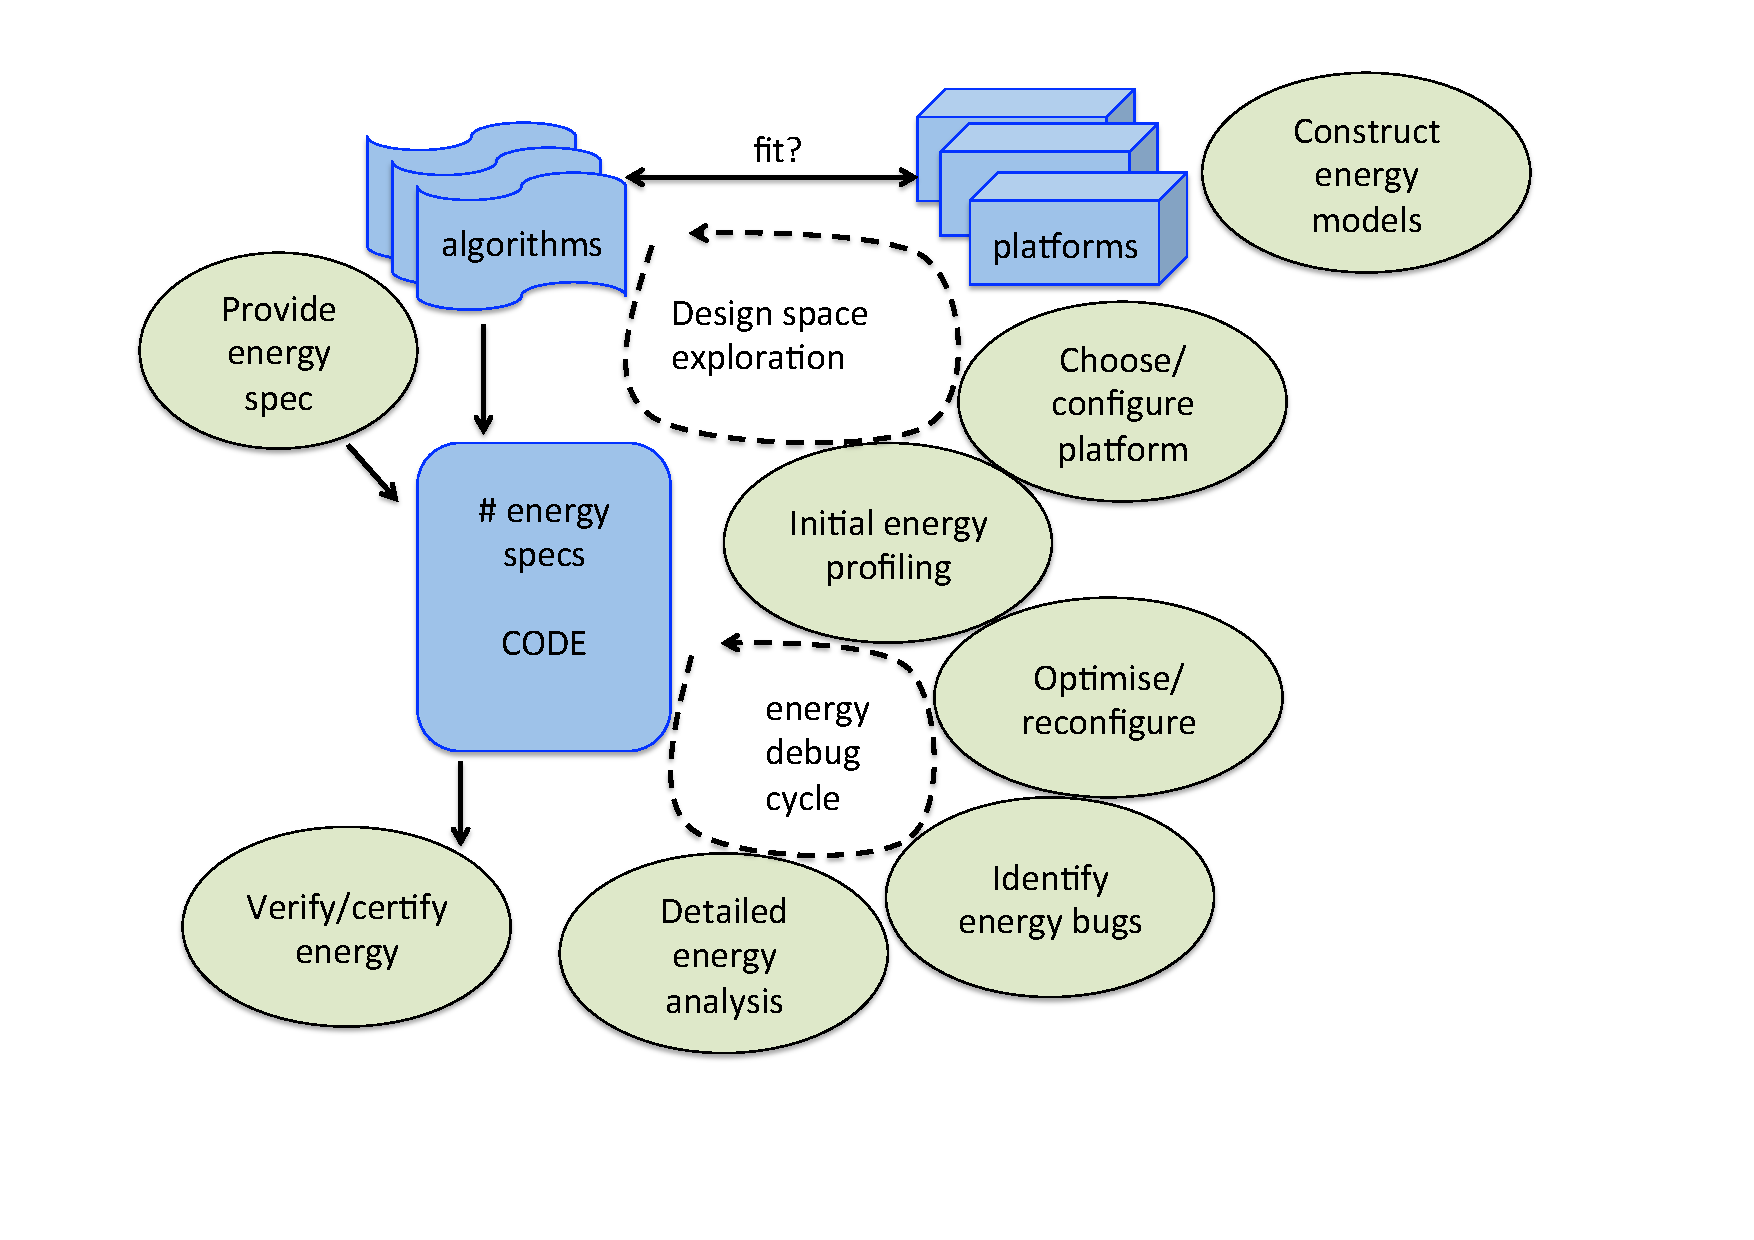
\includegraphics[width=14cm]{\figpath/EASWEngineering-slide}}
\vspace{-1.5cm}
\caption{Energy-aware software engineering activities.}
\label{fig:EASWEngineering}
\end{figure}


\subsection{Energy-aware software engineering activities}\label{sweng-activities}

In this section we describe the most important activities involved in
energy-aware software engineering.  Some of these activities are
extensions or modifications of conventional software engineering
practices; others are new activities that only exist when energy
efficiency is a design goal.  Figure \ref{fig:EASWEngineering} shows a
number of activities and (some of) the inter-dependencies that arise
in the context of different scenarios.

\subsubsection{Specify application, including energy}
The process of developing application software starts with a
requirements specification that expresses not only \emph{functional} properties, as
in the classical approach, but also \emph{non-functional} properties,
including energy consumption and other resources.  Classical
methods for requirements specification need to be extended to allow
non-functional specifications to be expressed. 

Satisfying
functional properties (in the sense of the classical concept of
correctness with respect to a test suite or a formal input-output
specification) is as important as doing so for non-functional
properties: an application that makes a device run out of batteries
before a task is completed is as erroneous and useless as an
application that does not compute the right result. 

\subsubsection{Construction of energy models}\label{energy-models}

Creating energy models for different combinations of hardware platforms and programming 
languages is a part of the energy-aware development process.  At one end of the 
spectrum,  one might
expect future hardware manufacturers to deliver an energy model for their instruction set architecture 
and thus the model would be available ``off the shelf".  At the other end, some
projects might require the construction of an energy model specific to that project, perhaps
because the hardware or software environment was not standard.  In between these two
extremes, energy modelling  for energy-aware software development is becoming a more
well understood process.

\subsubsection{Resource model of deployment platform}\label{platform-model}

If energy efficiency is a design goal, we need to obtain an \emph{energy model
of the platform} on which the system is to be deployed (even though the
software might be developed on a different platform).

Thus obtaining the appropriate energy model is a vital task in energy-aware 
software engineering.  Not only should an appropriate platform be selected, but
its energy model should be available during software development to support other 
activities (see for example Sections \ref{space-expl}, \ref{init-energy}, \ref{energy-analysis} and \ref{energy-bugs}).
We note also that several different energy models for a given platform might be
selected, at different levels of abstraction suitable for different activities.  For instance,
high-level approximate models might be suitable for design space exploration (Section \ref{space-expl}) and initial energy profiling (Section \ref{init-energy}), while more precise low-level models are needed for detailed energy analysis (Section \ref{energy-analysis}) and optimisation 
(Section \ref{energy-opt}).

\subsubsection{Selection of deployment platform}\label{platform-choice}

The choice of deployment platform itself might depend on its resource-usage model; thus 
this activity and Section \ref{platform-model} are interdependent.
By ``platform"
here is meant both the hardware and the software platform; thus the model
should be capable of predicting the energy usage of software (in a given language
and with a given runtime environment) 
being executed on a given piece of hardware.

\subsubsection{Configure platform}\label{platform-config}

Some platforms allow configuration that can have implications for energy consumption.
Among such settings are clock frequency and voltage, the
number of cores and the communication paths among them. At the software level,
operating system settings can also be considered, such as the settings for power saving 
and the resolution of OS
timer processes that can send interrupts to other processes.


\subsubsection{Design space exploration}\label{space-expl}

Choices taken early on in the design process can have a profound effect on the
energy efficiency of the final result.  \emph{Design space exploration} as an 
energy-aware software development activity refers to the process of estimating
energy implications of different possible design solutions, before they are implemented.
It may involve especially activities such as Selection of deployment platform (Section \ref{platform-choice}), Platform configuration (Section \ref{platform-config}) and Initial energy profiling (Section \ref{init-energy}).
This involves energy modelling and analysis tools as in some other activities, but
with the difference that one is likely to be more satisfied with approximate models
and thus rougher estimates
of energy consumption rather than precise predictions.

\subsubsection{Initial energy profiling}\label{init-energy}

At early stages of energy aware software design and implementation, tools are needed 
to perform an \emph{initial energy analysis}.  The purpose
of this is to produce statically an \emph{energy profile} that
identifies the overall
complexity of the energy consumption of the software and how energy consumption is
distributed over the parts of the program.   It could also at this stage identify
energy bugs (parts of the application software that do not meet
their energy consumption specification).

Initial energy analysis requires an
an \emph{energy model} of the deployment platform at an appropriate
level of abstraction. At early stages, parts of the software may be missing
and it might not be possible to compile it to machine instructions; thus
an approximate model based on a model of source code might have to
suffice.

\subsubsection{Detailed energy analysis}\label{energy-analysis}

During more advanced stages of energy aware software implementation,
detailed energy analyses at finer levels of granularity are needed.
These are provided by tools containing more precise low-level energy models 
of the platform, able to give precise estimates of the energy consumption
of critical parts of the code, which could be targets for energy optimisation.  


\subsubsection{Identify energy bugs}\label{energy-bugs}
Energy bugs occur when software does not conform to an energy specification.
The specification might state some overall resource requirement in which
energy consumption is implicit, for example on the length of battery life.  The
bug in such a case could be some energy-consuming process that is more
expensive than necessary, a service that is not switched off when required,
threads that synchronise badly and spend too much time waiting, and so on.


\subsubsection{Energy optimisation or reconfiguring}\label{energy-opt}

The broad concept of energy optimisation is applied throughout the whole software
engineering process, and starts
right at the beginning with design space exploration and selection of appropriate platform,
algorithms and data structures.

The specific energy optimisation performed in this activity 
is driven by the detailed energy analysis
and the energy model of the platform.  Both manual and automatic
optimisations can be applied; the energy analysis should point to the sections of
code that use the most energy, either because they involve costly energy operations,
or because they are frequently executed (e.g., tight inner loops).
This activity also includes application of energy-optimising compilers and such
generic optimisers.

\subsubsection{Verify or certify energy consumption}\label{certify}

Energy-critical applications need to be certified with respect to an
energy specification. Tools combining detailed energy models and
precise energy analysis are required in order to compare the inferred
energy consumption with the specification, either verifying conformance or 
certifying that it holds within some specified limits of behaviour such
as input ranges.


\subsection{Energy-aware software engineering scenarios}\label{sweng-scenarios}


In this section we sketch scenarios in which the activities described
in the previous section are applied.

\subsubsection{Embedded system development on xCORE}\label{xcore-scenario}

The ENTRA project case studies focussed on embedded systems implemented in the XC language and deployed on the xCORE multicore architecture.  An energy-aware software development strategy for such applications might involve the following energy-aware activities.
\begin{itemize}
\item
Energy specification by writing pragma comments in the XC source code.  Such pragmas could express energy constraints derived from customer requirements on the power supply.
\item
Platform selection and configuration.  The xCORE architecture is highly configurable both in terms of the number of cores and their interconnection.  The choice and configuration is guided by an energy model applied to proposed solutions, taking into account thread communication energy costs in a given configuration, as described in more detail in \cite{KerrisonSwallow15}).
\item
Detailed program-independent energy models of the platform at \isa\ level, are available.  
Program-dependent energy models are obtained for XC and \llvmir\ code for the application from the \isa\ model, and used to perform more precise and detailed energy analysis of the application.
\item
Optimisations of expensive or frequently executed code is performed on the basis of the energy analysis.
\item
The energy optimising compiler for XC is applied to the application.
\item
Pragmas in the code are verified using comparison of the energy consumption predicted by the analysis with the constraints in the specification.  

\end{itemize}


\subsubsection{Android app development}\label{android-scenario}

A case study on Android app energy optimisation was carried out \cite{LiGallagher-TSE-2016}.  The study involved  energy modelling and optimisation of applications based on an established game-engine.  An energy specification was not given; the aim of the study was to use a source-code-level energy model to identify the most energy-intensive parts of the code in a number of typical use-cases, and then apply manual optimisations, reducing energy usage directly and thus prolonging battery life.

Energy-aware software engineering activities included:
\begin{itemize}
\item
Building a fine-grained source code energy model by regression
analysis from energy measurements on the target hardware and Android
software platform of a set of test cases exercising the functions of
the underlying game engine.

\item

Dynamic profiling of the code, which provided an energy profile that
allowed the most energy-expensive basic blocks to be identified.

\item Manual refactoring of the source code, targeted at the most
  expensive blocks, which succeeded in increasing energy efficient by
  a factor of 6\% to 50\% in various use-case scenarios.
\end{itemize}

\bibliographystyle{alpha}
\bibliography{../../../ENTRA/entra-svn/bibtex/entra}

\end{document}
